% version 1.00, date 20/02/16, auteur Michel Cressant
Ce chapitre décrit les différents cas d'utilisation pour chaque fonctionnalité.


\section{Fonctionnalité 8}
Ce paragraphe décrit les cas d'utilisation concernant la fonctionnalité 8 soit l'attribution de frimousse. \\

La figure suivante (figure \ref{diagrammeCasUtilisation8}) indique les cas d'utilisation pour la géolocalisation.
\begin{figure}[H]
	\centering
	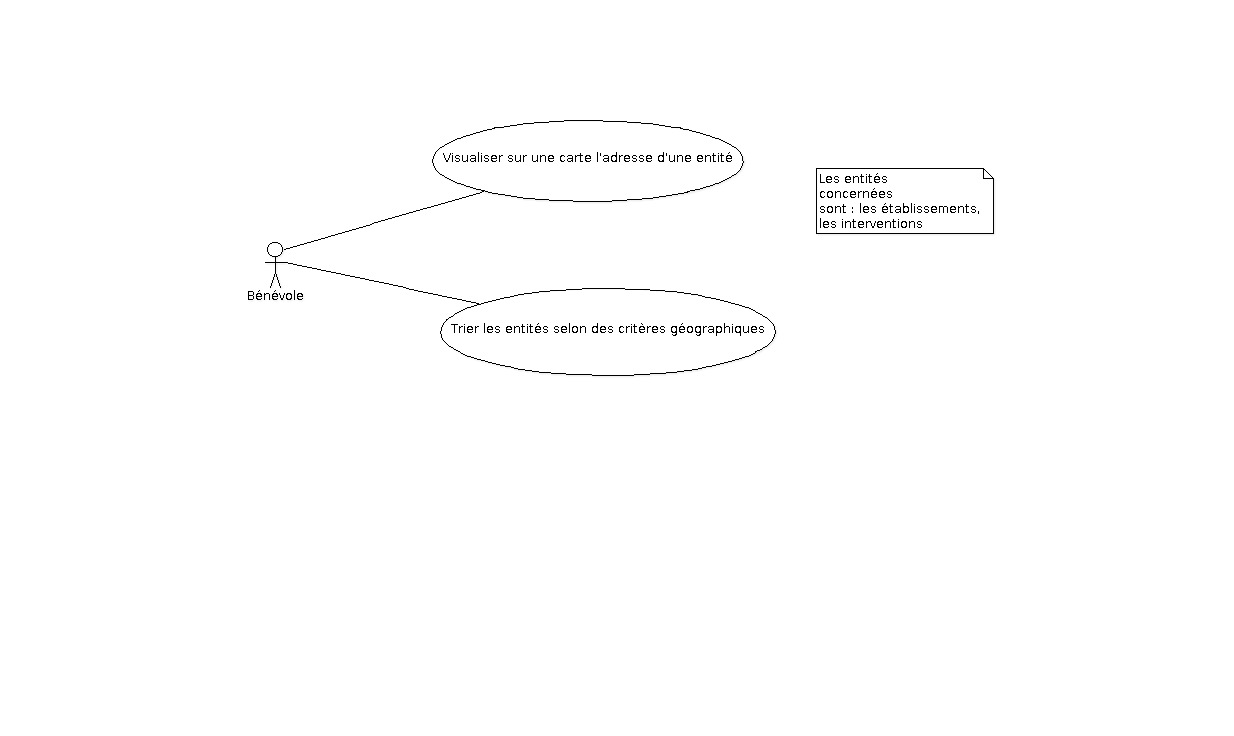
\includegraphics[scale=0.40]{casDUtilisation/images/fonctionnalite8Geolocalisation.png}
	\caption{Cas d'utilisation~: Géolocalisation }
	\label{diagrammeCasUtilisation8}
\end{figure}

\section{Fonctionnalité 9}
Ce paragraphe décrit les cas d'utilisation concernant la fonctionnalité 9 soit l'attribution de frimousse. \\

La figure suivante (figure \ref{diagrammeCasUtilisation9}) indique les cas d'utilisation pour l'attribution de frimousse.
\begin{figure}[H]
	\centering
	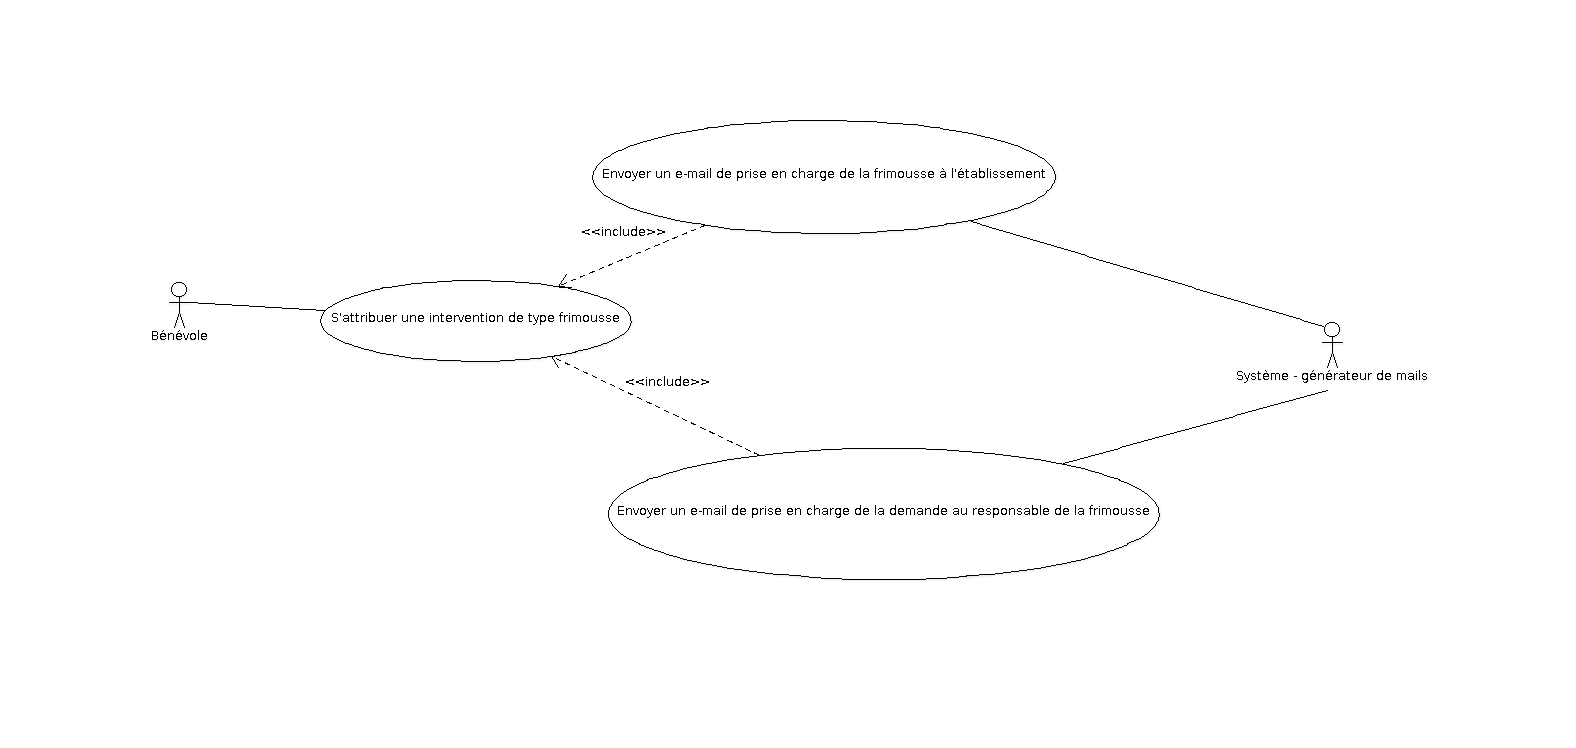
\includegraphics[scale=0.35]{casDUtilisation/images/fonctionnalite9Attribution.png}
	\caption{Cas d'utilisation~: Attribution de frimousse }
	\label{diagrammeCasUtilisation9}
\end{figure}

\section{Fonctionnalité 10}
Ce paragraphe décrit les cas d'utilisation concernant la fonctionnalité 10 soit la gestion des ventes. \\

La figure suivante (figure \ref{diagrammeCasUtilisation10}) indique les cas d'utilisation pour l'attribution de frimousse.
\begin{figure}[H]
	\centering
	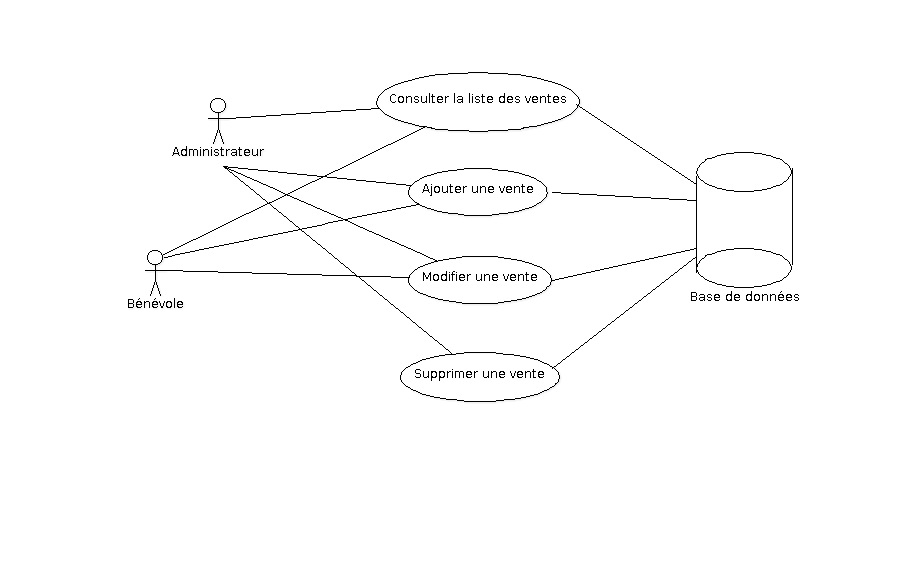
\includegraphics[scale=0.40]{casDUtilisation/images/fonctionnalite10Vente.png}
	\caption{Cas d'utilisation~: Gestion des ventes }
	\label{diagrammeCasUtilisation10}
\end{figure}
